\input{head.inc}
\usepackage{tikz-3dplot}
\usetikzlibrary{shapes.geometric}
\usepackage{pgfplots}
\pgfplotsset{compat = newest}
\usepackage[europeanresistors,americaninductors]{circuitikz}

% Präambelbefehle für die Präsentation
\title[TET: Wellenleiter II - Klassische Leitungstheorie]{TET: Wellenleiter II - Klassische Leitungstheorie}

\begin{document}
% 
% Frontmatter 
% 
%%%%%%%%%%%%%%%%%%%%%%%%%%%%%%%%%%%%%%%%%%%%%%%%%%%%%%%%%%%%%%%%%%%%%%%%%%%%%%%%%%%%%%%%%%%%%%%%%%%%%%%%%%%%%%%%%%%%%%%%%%%%% 

%% inserts the title page and the table of contents
\maketitle

% 
% Content 
% 
%%%%%%%%%%%%%%%%%%%%%%%%%%%%%%%%%%%%%%%%%%%%%%%%%%%%%%%%%%%%%%%%%%%%%%%%%%%%%%%%%%%%%%%%%%%%%%%%%%%%%%%%%%%%%%%%%%%%%%%%%%%%% 
\section{TET: Wellenleiter II - Klassische Leitungstheorie}

\begin{frame}
  \frametitle{Klassische Leitungstheorie}
  \begin{itemize}[<+->]
  \item Die \alert{klassische Leitungstheorie} dient der Beschreibung von \alert{langen Leitungen} mittels \alert{Strom und Spannung}.
  \item Von einer \alert{langen Leitung} spricht man, wenn die Länge der Leitung nicht mehr als klein im Vergleich zur \alert{Wellenlänge} angesehen werden kann.
    \centerline{%
    \begin{tabular}{c||c|c|c|c|c|c}
      $f$ & \SI{50}{\hertz} & \SI{1}{\kilo\hertz} & \SI{100}{\mega\hertz}& \SI{1}{\giga\hertz}& \SI{10}{\giga\hertz}\\
      \hline
      $\lambda_{\text{Vakuum}}=\frac{\lichtgeschw}{f}$ & \SI{5995.8}{\kilo\metre} & \SI{299.8}{\kilo\metre} &\SI{2.99}{\metre} &\SI{29.9}{\centi\metre}&\SI{2.9}{\centi\metre}
    \end{tabular}}
  \item Im einfachsten Fall wird die Leitung als \alert{verlustlose, homogene Einfachleitung} angesehen. Es handelt sich also um einen \alert{zylindrischen Wellenleiter}.
  \item Das Querschnittsgebiet ist \alert{nicht einfach zusammenhängend} und daher existiert ein (quasi) {TEM-Mode}.
  \item Nur der TEM-Mode wird betrachtet: daher kann mit \alert{Spannungen in der Transversalebene} gerechnet werden.
    \item Verallgemeinerungen bis hin zu einer \alert{full-wave} Beschreibung sind möglich!
  \item Beispielstrukturen, die gerne mit Leitungstheorie beschrieben werden:

    \begin{columns}[t]
      \begin{column}{.3\linewidth}
        Koaxialkabel
        
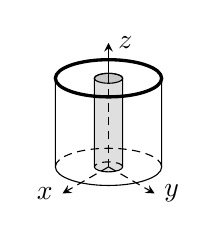
\begin{tikzpicture}[scale=.9]
  \draw [fill=gray, fill opacity=.25] (180:2mm) coordinate (a) 
  -- ++(0,-12.5mm) coordinate (b)
  arc (180:360:2mm and .7mm) coordinate (d) % 2 war 5
  -- (a -| d) coordinate (c) arc (0:180:2mm and .7mm); % 2 war 5
  \draw [fill=gray, fill opacity=.25]
  (0,0) coordinate (t) circle (2mm and .7mm);
  \draw [densely dashed] (d) arc (0:180:2mm and .7mm);
  \draw []
  (180:7.5mm) coordinate (A)
  -- ++(0,-12.5mm) coordinate (B) 
  arc (180:360:7.5mm and 2.625mm) coordinate (D)
  -- (A -| D) coordinate (C) arc (0:180:7.5mm and 2.625mm);
  \draw [very thick]
  (0,0) coordinate (T) circle (7.5mm and 2.625mm);
  \draw [densely dashed] (D) arc (0:180:7.5mm and 2.625mm);
  \draw [densely dashed ]
  ([yshift=-12.5mm]T) coordinate (B)
  edge [-stealth] node [pos=1, right] {$y$} +(-30:7.5mm)
  edge [-stealth] node [pos=1, left] {$x$} +(-150:7.5mm)
  -- (T) edge [solid, -stealth] node [right, pos=1] {$z$} ++(0,5mm) ;
\end{tikzpicture}

\end{column}
\begin{column}{.3\linewidth}
  Zweidrahtleitung (Lecher-Leitung)

  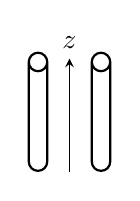
\begin{tikzpicture}[scale=.8]
\node [thick,cylinder, draw, shape border rotate=90,minimum height=1.5cm,minimum width=2mm] at (0,0){}; 
\node [thick,cylinder, draw, shape border rotate=90,minimum height=1.5cm,minimum width=2mm] at (1cm,0cm){};
\draw[thin, -stealth] (0.5cm,-0.80cm) -- (0.5cm,1cm) node[above]{$z$};
\end{tikzpicture}

        \end{column}
        \begin{column}{.3\linewidth}
          Mikrostreifenleitung
\bigskip
          
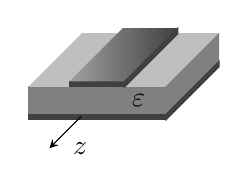
\begin{tikzpicture}[scale=0.35]
  \draw [lightgray] (0,1,0) coordinate (bl) -- (5,1,0) coordinate (br);
  \filldraw [gray] (0,0,5) coordinate (fll) -- (0,1,5) coordinate (ftl) -- (5,1,5) coordinate (ftr) -- (5,0,5) coordinate (flr) -- cycle;
  \shade [left color = lightgray, right color = lightgray] (bl) -- (br) -- (ftr) -- (ftl) -- cycle;
  \filldraw [gray] (5,0,0) coordinate (blr) -- (flr) -- (ftr) -- (br);
  \filldraw [darkgray] (fll) rectangle (5,-0.2,5) coordinate (flr2);
  \filldraw [darkgray] (flr2) -- (5,-0.2,0) coordinate (blr2) -- (blr) -- (flr) -- cycle;
  \filldraw [darkgray] (1.5,1.2,5) coordinate (ftl-1) -- (3.5,1.2,5) coordinate (ftr-1) -- (3.5,1,5) coordinate (flr-1) -- (1.5,1,5) coordinate (fll-1) -- cycle;
  \shade [left color = darkgray!50, right color = darkgray] (1.5,1.2,0) coordinate (btl-1) -- (3.5,1.2,0) coordinate (btr-1) -- (ftr-1) -- (ftl-1) -- cycle;
  \filldraw [darkgray] (flr-1) -- (ftr-1) -- (btr-1) --  (br -| btr-1) -- cycle;
  \node at (4,0.5,5) {$\varepsilon$};
  \coordinate (nA1) at (1.5,2.5,0);
  \coordinate (nB1) at (3.5,2.5,0);
  \coordinate (nA2) at (-1.5,1.2,0);
  \coordinate (nB2) at (-1.5,1.2,5);
  \coordinate (nA3) at (7,1,5);
  \coordinate (nB3) at (7,1.2,5);
  \coordinate (nA4) at (-1.5,1,5);
  \coordinate (nB4) at (-1.5,0,5);
  \draw[-stealth,thin] (0,-2,0) -- (0,-2,3) node[right,xshift=5]{$z$};
\end{tikzpicture}
        \end{column}
      \end{columns}
    \end{itemize}
    \ 
\end{frame}


\begin{frame}
  \frametitle{Ausgangspunkt}
  \begin{itemize}[<+->]
  \item Ziel ist die Entwicklung eines \alert{Ersatzschaltbilds} für ein \alert{differentielles Leitungselement}.
  \item Ausgangspunkt ist feldtheoretische Beschreibung für den \alert{verlustlosen Fall}.
  \item Das Ersatzschaltbild kann dann einfach \alert{verallgemeinert} werden.
  \item Maxwellgleichungen (lin. hom. iso. Dielektrikum, harmonische ZA, keine Quellen):
    \begin{align*}
      \divergenz \efeld[uv] &= 0 & \rotation\efeld[uv] + \komplex\omega\mu \magfeld[uv] &=\vec{0} \\
      \divergenz \magfeld[uv] &= 0 & \rotation\magfeld[uv] - \komplex\omega\varepsilon \efeld[uv] &=\vec{0} 
    \end{align*}
  \item Wir betrachten nur den \alert{TEM-Mode}. Die \alert{Ausbreitungsrichtung} sei \(\pm\einheitsvek{z}\). Es gilt:
    \begin{align*}
      \text{TEM-Mode: } && \efeld[uv]\cdot \einheitsvek{z} &=0 & \magfeld[uv]\cdot \einheitsvek{z} &=0 \\
                        && \left( \rotation \efeld[uv]\right)\times\einheitsvek{z} &= \frac{\d \efeld[uv]}{\d z} & \left( \rotation \magfeld[uv]\right)\times\einheitsvek{z} &= \frac{\d \magfeld[uv]}{\d z}
    \end{align*}
    \begin{equation*}
            \text{Transversalebene: }  \rotation_t\efeld[uv] = \left( \frac{\d \efeld[u]_y}{\d x}-\frac{\d \efeld[u]_x}{\d y}\right)\einheitsvek{z} \Rightarrow\left(\rotation_t\efeld[uv]\right)\cdot\einheitsvek{x,y} =0
    \end{equation*}                                                                                                    
    \end{itemize}
\end{frame}

\begin{frame}
  \frametitle{Felder -- Transversalebene (\(z=\text{const.}\))}
  \begin{itemize}[<+->]
  \item Transversalkomponente des Induktionsgesetztes (in der Transversalebene):
    \begin{align*}
      \rotation \efeld[uv] + \komplex\omega\mu\magfeld[uv] &=\vec{0} \Rightarrow& \left(\rotation \efeld[uv]\right)\times\einheitsvek{z} + \komplex\omega\mu\magfeld[uv] \times\einheitsvek{z} &=\vec{0} \\
      && \Aboxed{\frac{\d \efeld[uv]}{\d z} + \komplex\omega\mu\magfeld[uv] \times\einheitsvek{z} &=\vec{0}} 
      \end{align*}
    \item Das elektrische Feld ist ein \alert{Gradientenfeld} in allen Transversalebenen. Ansatz:
      \begin{equation*}
        \boxed{\efeld[uv] = -\gradient\elpotential(x,y) \; g(z)} \text{ mit } \boxed{\laplace\elpotential(x,y) = 0} \text{ statische 2D Laplace Gleichung}
        \end{equation*}
      \item Magnetfeld direkt ausrechnen:
        \begin{align*}
          \frac{\d \efeld[uv]}{\d z} + \komplex\omega\mu\magfeld[uv] \times\einheitsvek{z} &=\vec{0} &\Rightarrow \einheitsvek{z}\times\frac{\d \efeld[uv]}{\d z} &+ \komplex\omega\mu\, \einheitsvek{z}\times\left(\magfeld[uv] \times\einheitsvek{z}\right) =\vec{0}\\
                                                                                           && \magfeld[uv] &= -\frac{1}{\komplex\omega\mu} \left(\einheitsvek{z}\times\frac{\d \efeld[uv]}{\d z}\right) \\
          &&\Aboxed{\magfeld[uv]&= \frac{1}{\komplex\omega\mu} \left(\einheitsvek{z}\times\gradient\elpotential\right)\frac{\d g}{\d z}}
\end{align*}
\end{itemize}
\end{frame}

\begin{frame}
  \frametitle{Übergang zu Strom und Spannung}
  \begin{columns}
    \begin{column}{.3\linewidth}
      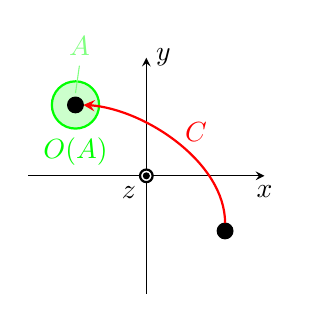
\begin{tikzpicture}
        \draw[thin,-stealth] (-1.5,0) -- (+1.5,0) node[below]{$x$};
        \draw[thin,-stealth] (0,-1.5) -- (0,+1.5) node[right]{$y$};
        \draw[fill=black] (1,-0.7) circle (0.1); 
        \draw[fill=green!20,draw=green,thick] (-0.9,0.9) circle (0.3) node[color=green,below,yshift=-8]{$O(A)$}; 
        \draw[fill=black] (-0.9,0.9) circle (0.1); 
        \draw[thick,red,-stealth] (1,-0.6) .. controls (1,.2) and (-0.1,0.9) .. (-0.8,0.9) node[midway,right,yshift=3] {$C$};
        \draw[color=green!50] (-0.9,1.05) -- (-0.85,1.4) node[color=green!50,above]{$A$};
        \draw[thick, fill=white] (0,0) circle (0.08) node[anchor=north east]{$z$}; 
        \draw[thick, fill=black] (0,0) circle (0.03); 
        \end{tikzpicture}
      \end{column}
    \begin{column}{.7\linewidth}
  \begin{itemize}[<+->]
  \item Stromdichte konstant im Leiterquerschnitt \(\to\) \alert{Dünndrahtnäherung}
  \item Perfekte Leiter: \(\kappa \to \infty\)
  \item Rotationsfreiheit des elektrischen Felds in der Transversalebene \(\to\) \alert{Spannung}:
    \begin{equation*}
      \spannung[u] = \int_C \efeld[uv] \cdot \upd \vec{s} \; \text{ mit \(z =\) const. auf \(C\)}
    \end{equation*}
  \item Aus dem Durchflutungsgesetz \(\to\) \alert{Strom:}
    \begin{equation*}
      \elstrom[u] = \oint_{O(A)} \magfeld[uv] \cdot \upd\vec{s}
      \end{equation*}
  \end{itemize}
      \end{column}
  \end{columns}
  \begin{itemize}[<+->]
  \item Damit können die Ausdrücke für die Felder umgeformt werden:
          \begin{equation*}
        \frac{\d \efeld[uv]}{\d z} + \komplex\omega\mu\magfeld[uv] \times\einheitsvek{z} =\vec{0} \quad\text{und}\quad \magfeld[uv]= \frac{1}{\komplex\omega\mu} \left(\einheitsvek{z}\times\gradient\elpotential\right)\frac{\d g}{\d z} 
    \end{equation*}
    
  \end{itemize}
\end{frame}

\begin{frame}
  \frametitle{Übergang zu Strom und Spannung (\dots)}
  \begin{itemize}[<+->]
  \item Ausdrücke für die Felder:
          \begin{equation*}
        \frac{\d \efeld[uv]}{\d z} + \komplex\omega\mu\magfeld[uv] \times\einheitsvek{z} =\vec{0} \quad\text{und}\quad \magfeld[uv]= \frac{1}{\komplex\omega\mu} \left(\einheitsvek{z}\times\gradient\elpotential\right)\frac{\d g}{\d z} 
      \end{equation*}
      \item Wir bilden das Wegintegral der ersten Gleichung entlang \(C\) und setzen dann \(\magfeld[uv]\) ein: 
          \begin{align*}
            \int_C \frac{\d \efeld[uv]}{\d z} \cdot \upd \vec{s} + \komplex\omega\mu \int_C\left(\magfeld[uv] \times\einheitsvek{z}\right) \cdot \upd \vec{s} &= 0  \\
            \Aboxed{\frac{\d \spannung[u]}{\d z} + \frac{\d g}{\d z} \int_C\gradient\elpotential \cdot \upd \vec{s} = 0} 
          \end{align*}
        \item Weiter gilt für den Strom:
          \begin{align*}
            \elstrom[u] = \oint_{O(A)} \magfeld[uv] \cdot \upd\vec{s} &= \oint_{O(A)} \frac{1}{\komplex\omega\mu} \left(\einheitsvek{z}\times\gradient\elpotential\right)\frac{\d g}{\d z} \cdot \upd\vec{s}\\
                                                                        \Rightarrow \Aboxed{\frac{\d g}{\d z} &= \komplex\omega\mu \frac{\elstrom[u]}{\oint_{O(A)} \left(\einheitsvek{z}\times\gradient\elpotential\right) \cdot \upd\vec{s}}}
            \end{align*}
  \end{itemize}
\end{frame}

\begin{frame}
  \frametitle{Übergang zu Strom und Spannung (\dots)}
  \begin{itemize}[<+->]
  \item Wir betrachten die Formeln
    \begin{equation*}
      \frac{\d \spannung[u]}{\d z} + \frac{\d g}{\d z} \int_C\gradient\elpotential \cdot \upd \vec{s} = 0 \text{ und } \frac{\d g}{\d z} = \komplex\omega\mu \frac{\elstrom[u]}{\oint_{O(A)} \left(\einheitsvek{z}\times\gradient\elpotential\right) \cdot \upd\vec{s}}
    \end{equation*}
  \item Einsetzen der rechten in die linke Gleichung eliminiert offensichtlich die unbekannte Funktion \(g(z)\) und wie erhalten die \alert{erste Leitungsgleichung} (Telegraphengleichung):
    \begin{equation*}
      \frac{\d \spannung[u](z)}{\d z} + \komplex\omega \underbrace{\frac{\mu\int_C\gradient\elpotential \cdot \upd \vec{s}}{\oint_{O(A)} \left(\einheitsvek{z}\times\gradient\elpotential\right) \cdot \upd\vec{s}}}_{L^\prime} \elstrom[u](z)=\boxed{\frac{\d \spannung[u](z)}{\d z} + \komplex\omega L^\prime \elstrom[u](z)= 0} \quad [L^\prime] = \si{\henry\per\metre}
    \end{equation*}
\item Der \alert{Induktivitätsbelag} der Leitung \(L^\prime\) ist vollständig bestimmt durch die Lösung des statischen 2D Laplace-Randwertproblems für \(\elpotential\) im Lösungsvolumen \(V\)
  \begin{equation*}
    \laplace\elpotential(x,y) = 0 \text{ mit }  \elpotential = 0 \text{ auf einem Leiter und } \elpotential = \spannung(z) \text{ auf dem anderen Leiter}
    \end{equation*}
  \end{itemize}
\end{frame}


\begin{frame}
  \frametitle{Übergang zu Strom und Spannung (\dots)}
  \begin{itemize}[<+->]
  \item Analog folgt die \alert{zweite Leitungsgleichung} aus den Formeln:
          \begin{equation*}
        \frac{\d \magfeld[uv]}{\d z} - \komplex\omega\varepsilon\efeld[uv] \times\einheitsvek{z} =\vec{0} \text{ und } \efeld[uv] = -\gradient\elpotential \; g(z)
      \end{equation*}
      \item Umlaufintegral der ersten Gleichung entlang \(O(A)\) und Einsetzen von \(\efeld[uv]\) ergibt: 
          \begin{align*}
            \oint_{O(A)} \frac{\d \magfeld[uv]}{\d z} \cdot \upd \vec{s} - \komplex\omega\varepsilon \oint_{O(A)}\left(\efeld[uv] \times\einheitsvek{z}\right) \cdot \upd \vec{s} &= 0  \\
            \frac{\d \elstrom[u]}{\d z} -\komplex\omega\varepsilon\; g(z) \oint_{O(A)}\left(\einheitsvek{z}\times \gradient\elpotential\right) \cdot \upd \vec{s} &= 0 
          \end{align*}
        \item Die Funktion \(g(z)\) folgt sofort aus \(\spannung[u]\):
          \begin{equation*}
\spannung[u] = \int_C \efeld[uv]\cdot\upd\vec{s} = -g(z) \int_C \gradient\elpotential\cdot\upd\vec{s} \to g(z) = -\frac{\spannung[u]}{\int_C \gradient\elpotential\cdot\upd\vec{s}}
\end{equation*}
\item Damit lautet die \alert{zweite Leitungsgleichung}:
  \begin{equation*}
    \frac{\d \elstrom[u]}{\d z} +\komplex\omega \underbrace{\frac{\varepsilon\oint_{O(A)}\left(\einheitsvek{z}\times \gradient\elpotential\right) \cdot \upd \vec{s}}{\int_C \gradient\elpotential\cdot\upd\vec{s}}}_{C^\prime} \spannung[u] = 0 \quad [C^\prime]=\si{\farad\per\metre}
    \end{equation*}
  \end{itemize}
\end{frame}

\begin{frame}
  \frametitle{Leitungsgleichungen -- Leitungsbeläge}
  \begin{itemize}[<+->]
  \item Zusammenfassend haben wir für verlustlose Leitungen die folgenden \alert{Leitungsgleichungen} gefunden:
    \begin{align*}
      \frac{\d \spannung[u](z)}{\d z} + \komplex\omega L^\prime \elstrom[u](z) &= 0 & L^\prime &=\frac{\mu\int_C\gradient\elpotential \cdot \upd \vec{s}}{\oint_{O(A)} \left(\einheitsvek{z}\times\gradient\elpotential\right) \cdot \upd\vec{s}}\\
      \frac{\d \elstrom[u](z)}{\d z} +\komplex\omega C^\prime \spannung[u](z) & = 0 & C^\prime &= \frac{\varepsilon\oint_{O(A)}\left(\einheitsvek{z}\times \gradient\elpotential\right) \cdot \upd \vec{s}}{\int_C \gradient\elpotential\cdot\upd\vec{s}}
    \end{align*}
  \item Offensichtlich gilt
    \begin{equation*}
      L^\prime C^\prime = \varepsilon\mu = \frac{1}{\geschw_p^2} \Rightarrow \boxed{\geschw_p = \frac{1}{\sqrt{L^\prime C^\prime}}}
    \end{equation*}
  \item Entkoppelte Gleichungen:
    \begin{equation*}
      \frac{\d^2 \spannung[u](z)}{\d z^2} + \omega^2 L^\prime C^\prime \spannung[u](z) = 0 \text{ und } \frac{\d^2 \elstrom[u](z)}{\d z^2} + \omega^2 L^\prime C^\prime \elstrom[u](z) = 0
    \end{equation*}
  \item Die Lösungen sind (natürlich) vor- und zurücklaufende Wellen (als ruhende Zeiger):
    \begin{equation*}
      \spannung[u](z) = \spannung[u]_0 \euler^{\pm\komplex kz} \text{ und } \elstrom[u](z) = \elstrom[u]_0 \euler^{\pm\komplex kz}
      \end{equation*}
  \end{itemize}
\end{frame}

\begin{frame}
  \frametitle{Übergang zum Ersatzschaltbild}
  \begin{columns}
    \begin{column}{.4\linewidth}
    \ctikzset{voltage/bump b=1.1}
  \begin{circuitikz}[european voltages,scale=.75]
\draw (0,0) to[short,o-o] (4,0);
\draw (0,2) to [short, i=$\underbar{I}(z)$,o-] (1,2) to[L=L,-] (3,2) coordinate(a);
\draw (a) to[short, i=$\underbar{I}(z+\Delta z)$,-o]  (4,2);
\draw (a) to[C,l_=C,*-*] ++(0,-2);
 
% Voltage labels
\draw (0,2) to[open,v=$\underbar{U}(z)$] ++(0,-2);
\draw (4,2) to[open, v^=$\underbar{U}(z+\Delta z)$] ++(0,-2);
\end{circuitikz}
\end{column}
\begin{column}{.6\linewidth}
  \begin{itemize}[<+->]
  \item Maschensatz:
    \begin{align*}
      \spannung[u](z) = \komplex\omega L \elstrom[u](z) + \spannung[u](z+\Delta z)\\
      \spannung[u](z+\Delta z) -\spannung[u](z) + \komplex\omega L \elstrom[u](z) =0  \\
      \frac{\Delta \spannung[u]}{\Delta z} + \komplex\omega \frac{L}{\Delta z} \elstrom[u](z) =0
      \end{align*}
  \end{itemize}
\end{column}
\end{columns}
  \begin{itemize}[<+->]
  \item Knotensatz:
    \begin{equation*}
      \elstrom[u](z+\Delta z) = \elstrom[u](z) - \komplex\omega C \spannung[u](z+\Delta z) \Rightarrow \frac{\Delta \elstrom[u]}{\Delta z} + \komplex\omega \frac{C}{\Delta z} \spannung[u](z+\Delta z) = 0   
    \end{equation*}
  \item Im Grenzfall \(\Delta z \to 0\) und mit \(C^\prime=\lim_{\Delta z \to 0} \frac{C}{\Delta z}\) und \(L^\prime=\lim_{\Delta z \to 0} \frac{L}{\Delta z}\) ist der obige Vierpol das \alert{Ersatzschaltbild eines differentiellen Stückes einer verlustlosen Leitung.}
    \item Verallgemeinerung für \alert{verlustbehaftete} Leitungen:
      \ctikzset{voltage/bump b=1.1}
      \ctikzset{bipoles/length=.7cm}
  \begin{circuitikz}[european voltages,scale=.75]
\draw (0,0) to[short,o-o] (7,0);
\draw (0,1.5) to [short, i=$\underbar{I}(z)$,o-] (1,1.5) to[R=$R^\prime \upd z$] (2,1.5) to[L=$L^\prime \upd z$,-] (4,1.5) coordinate(a);
\draw (a) to[short, -] (5,1.5) coordinate(b);
\draw (b) to[short, i=$\underbar{I}(z+\upd z)$,-o]  (7,1.5);
\draw (a) to[C,l_=$C^\prime \upd z$,*-*] ++(0,-1.5); 
\draw (b) to[R,l=$G^\prime \upd z$,*-*] ++(0,-1.5); 
 
% Voltage labels
\draw (0,1.5) to[open,v=$\underbar{U}(z)$] ++(0,-1.5);
\draw (7,1.5) to[open, v^=$\underbar{U}(z+\upd z)$] ++(0,-1.5);
\end{circuitikz}
\end{itemize}
\ 
\end{frame}

\begin{frame}
  \frametitle{Verlustbehaftete Leitungen}
  \begin{center}
      \ctikzset{voltage/bump b=1.1}
      \ctikzset{bipoles/length=.7cm}
  \begin{circuitikz}[european voltages,scale=.75]
\draw (0,0) to[short,o-o] (7,0);
\draw (0,1.5) to [short, i=$\underbar{I}(z)$,o-] (1,1.5) to[R=$R^\prime \upd z$] (2,1.5) to[L=$L^\prime \upd z$,-] (4,1.5) coordinate(a);
\draw (a) to[short, -] (5,1.5) coordinate(b);
\draw (b) to[short, i=$\underbar{I}(z+\upd z)$,-o]  (7,1.5);
\draw (a) to[C,l_=$C^\prime \upd z$,*-*] ++(0,-1.5); 
\draw (b) to[R,l=$G^\prime \upd z$,*-*] ++(0,-1.5); 
 
% Voltage labels
\draw (0,1.5) to[open,v=$\underbar{U}(z)$] ++(0,-1.5);
\draw (7,1.5) to[open, v^=$\underbar{U}(z+\upd z)$] ++(0,-1.5);
\end{circuitikz}
\end{center}
  \begin{itemize}[<+->]
    \item Aus dem Ersatzschaltbild ergeben sich die \alert{Leitungsgleichungen für verlustbehaftete Leitungen}. 
    \begin{align*}
      \frac{\d \spannung[u](z)}{\d z} + \left(R^\prime + \komplex\omega L^\prime\right) \elstrom[u](z) &= 0 & L^\prime &=\frac{\mu\int_C\gradient\elpotential \cdot \upd \vec{s}}{\oint_{O(A)} \left(\einheitsvek{z}\times\gradient\elpotential\right) \cdot \upd\vec{s}}\\
      \frac{\d \elstrom[u](z)}{\d z} +\left(G^\prime + \komplex\omega C^\prime\right) \spannung[u](z) & = 0 & C^\prime &= \frac{\varepsilon\oint_{O(A)}\left(\einheitsvek{z}\times \gradient\elpotential\right) \cdot \upd \vec{s}}{\int_C \gradient\elpotential\cdot\upd\vec{s}}
    \end{align*}
  \item Der \alert{Widerstandsbelag} \(R^\prime\) entspricht den ohmschen Leitungsverlusten pro Längeneinheit.
  \item Der \alert{Leitwertbelag} \(G^\prime\)  entspricht den dielektrischen Verlusten pro Längeneinheit.
    \item Zusammengefasst spricht man auch vom \alert{Impedanzbelag} \(Z^\prime = R^\prime + \komplex\omega L^\prime\) und vom \alert{Admittanzbelag} \(Y^\prime = G^\prime + \komplex\omega C^\prime\) 
    \end{itemize}
\ 
  \end{frame}

  \begin{frame}
    \frametitle{Allgemeine Lösung -- Leitungswellenwiderstand}
      \begin{itemize}[<+->]
      \item Wir können die entkoppelten Leitungsgleichungen jetzt auch allgemein hinschreiben:
    \begin{equation*}
      \frac{\d^2 \spannung[u](z)}{\d z^2} -  Z^\prime Y^\prime \spannung[u](z) = 0 \text{ und } \frac{\d^2 \elstrom[u](z)}{\d z^2} -  Z^\prime Y^\prime \elstrom[u](z) = 0
    \end{equation*}
  \item Ansatz:
    \begin{equation*}
      \spannung[u](z) = u \euler^{\pm\gamma z} \Rightarrow \gamma = \sqrt{Z^\prime Y^\prime} = \sqrt{\left(R^\prime + \komplex\omega L^\prime\right) \left(G^\prime + \komplex\omega C^\prime\right)} \text{ Ausbreitungskonstante}
    \end{equation*}
  \item Mit der Spannung \(\spannung[u](z) = u_1 \euler^{-\gamma z} + u_2 \euler^{\gamma z}\) ergibt sich der Strom zu
    \begin{equation*}
      \elstrom[u](z) = - \frac{1}{Z^\prime} \frac{\d \spannung[u](z)}{\d z} = \frac{\gamma}{Z^\prime} \left( u_1 \euler^{-\gamma z} - u_2 \euler^{\gamma z}\right) = \frac{1}{Z_L} \left( u_1 \euler^{-\gamma z} - u_2 \euler^{\gamma z}\right)  
    \end{equation*}
  \item Hierbei ist \(Z_L\) der \alert{Leitungswellenwiderstand}:
    \begin{equation*}
      Z_L= \frac{Z^\prime}{\gamma} = \sqrt{\frac{Z^\prime}{Y^\prime}} = \sqrt{\frac{R^\prime + \komplex\omega L^\prime}{G^\prime + \komplex\omega C^\prime}} 
    \end{equation*}
    \item Abschluss mit Leitungswellenwiderstand \(\to\) Eingangsimpedanz = Leitungswellenwiderstand \(\to\) \alert{keine Reflexion}
    \end{itemize}
    \ 
  \end{frame}
  
  \begin{frame}
    \frametitle{Matrixschreibweise -- Mehrfachleitungen}
      \begin{itemize}[<+->]
      \item Die gefundenen Leitungsgleichungen werden üblicherweise in eine \alert{Matrixgleichung} zusammengefasst:
        \begin{equation*}
          \left.
    \begin{array}{rl}
      \frac{\d \spannung[u](z)}{\d z} + \left(R^\prime + \komplex\omega L^\prime\right) \elstrom[u](z) &= 0 \\
      \frac{\d \elstrom[u](z)}{\d z} +\left(G^\prime + \komplex\omega C^\prime\right) \spannung[u](z)  &= 0 
    \end{array}\right\} \Rightarrow
  \frac{\d}{\d z}\begin{pmatrix}\spannung[u](z)\\\elstrom[u](z) \end{pmatrix}
  +
  \begin{pmatrix}
    0 & Z^\prime \\
    Y^\prime & 0
  \end{pmatrix}
  \begin{pmatrix}\spannung[u](z)\\\elstrom[u](z) \end{pmatrix} = 0
\end{equation*}
\item Die Matrixgleichung ist sofort für \alert{Mehrfachleitungen} verallgemeinbar. Hierzu bilden wir
  \begin{itemize}[<+->]
    \item den Vektor der Spannungen relativ zum Bezugsleiter \(\vec{\spannung[u]}(z) = \left(\spannung[u]_1(z),\ldots , \spannung[u]_n(z) \right)^T\). 
    \item den Vektor der Ströme im Leiter  \(\vec{\elstrom[u]}(z) = \left(\elstrom[u]_1(z),\ldots , \elstrom[u]_n(z) \right)^T\).
    \item die Matrix mit den Impedanzbelägen in der Hauptdiagonalen \(\left(Z^\prime\right)\) 
    \item die Matrix mit den Admittanzbelägen in der Hauptdiagonalen \(\left(Y^\prime\right)\) 
\begin{equation*}
  \frac{\d}{\d z}\begin{pmatrix}\vec{\spannung[u]}(z)\\\vec{\elstrom[u]}(z) \end{pmatrix}
  +
  \begin{pmatrix}
    0 & \left(Z^\prime\right) \\
    \left(Y^\prime\right)^\prime & 0
  \end{pmatrix}
  \begin{pmatrix}\vec{\spannung[u]}(z)\\\vec{\elstrom[u]}(z) \end{pmatrix} = 0
\end{equation*}

    \end{itemize}
  \end{itemize} 
  \end{frame}

  \begin{frame}
    \frametitle{Bemerkungen}
      \begin{itemize}[<+->]
      \item Die Leitungstheorie kann hier nur angerissen werden.
      \item Die Anwendungen sind extrem vielfältig: Beschreibung von Leitungen, Impedanztransformationen, Anpassungen, Filter, \dots
        \item Vierpolparameter: Z, S, Y \(\to\) bekannt aus Grundlagen (Vierpole)
      \item \alert{Ungleichförmige Leitungen}: ortsabhängigen Leitungsbeläge
      \item Wichtigste Einschränkung der klassischen Leitungstheorie: \alert{nur TEM-Mode}
      \item Deshalb auch: Abstrahlung und Einkopplung in Leitungen nur bedingt beschreibbar.
        \item Lösung: \alert{Transmission Line Super Theory (TLST)}, z.B. F. Ossevorth, R. Jacobs, H.G. Krauthäuser,
\enquote{A full wave description for thin wire structures with TLST and perturbation theory}, Advances in Radio Science (16), 123--133, 2018. \url{https://ars.copernicus.org/articles/16/123/2018/}, DOI = 10.5194/ars-16-123-2018 und dort zitierte Arbeiten (insbesondere: S. Tkachenko und J. Nitsch)
  \end{itemize} 
  \end{frame}


        
\input{finalframe.inc}
   
\end{document}